\documentclass[parskip=full, a4paper]{scrartcl}

%%% PACKAGES %%%

% add unicode support and use german as language
\usepackage[utf8]{inputenc}
\usepackage[ngerman]{babel}

% Use Helvetica as font
\usepackage[scaled]{helvet}
\renewcommand\familydefault{\sfdefault}
\usepackage[T1]{fontenc}

% Better tables
\usepackage{tabularx}

% Better enumerisation env
\usepackage{enumitem}

% Use graphics
\usepackage{graphicx}

% Have subfigures and captions
\usepackage{subcaption}

% Be able to include PDFs in the file
\usepackage{pdfpages}

% Have custom abstract heading
\usepackage{abstract}

% Better equation environment
\usepackage{amsmath}

% Symbols for most SI units
\usepackage{siunitx}

\usepackage{csquotes}

% Clickable Links to Websites and chapters
\usepackage{hyperref}

% Code Highlighting
\usepackage{listings}
\lstset{language=XML}

%%% Not clearpage before chapter
\usepackage{etoolbox}
\makeatletter
\patchcmd{\scr@startchapter}{\if@openright\cleardoublepage\else\clearpage\fi}{}{}{}
\makeatother

%%% FALLBACK DocumentVersion if local build
\providecommand{\docversion}{0.0-localBuild}

%%% PATH DEFINITIONS %%%
% Define the path were images are found
\graphicspath{{./img/}{./pdf/}}

%%% DOCUMENT %%%

\begin{document}
\begin{titlepage}
\vspace*{2.5cm}
\noindent
\Huge{\textbf{Bericht des Tests der Referenzimplementation}} \\
\noindent
\Large{28.05.2019, Büron}\\
\vfill
\noindent
\large{Autor: Pascal Baumann}\\
\noindent
\large{Datum: \today}\\
\noindent
\large{Version: \docversion}\\
\end{titlepage}

\tableofcontents
\clearpage

\section{Einleitung}
Die im Sprint 07 entwickelte Referenzimplementation wurde am 28.05.2019 in der Speicherbibliothek in Büron getestet. Dafür wurden drei Laptops, zwei Antennen, ein Lesegerät und eigens dafür entwickelte Halterung eingeladen und nach Büron mitgenommen. Vor Ort entdeckte das Team, dass der Test in der Produktivumgebung unter Vollast laufen wird, und nicht auf einem separaten Förderband. Dies führte zu einer gewissen Anspannung beim Aufbau, da das Team auf keinen Fall die Mitarbeiteten belästigen und beeinträchtigen oder die Maschinerie beschädigen wollte (vergleiche Abbildung \ref{fig:AufbauSensorik}).

\begin{figure}[htb]
	\centering
	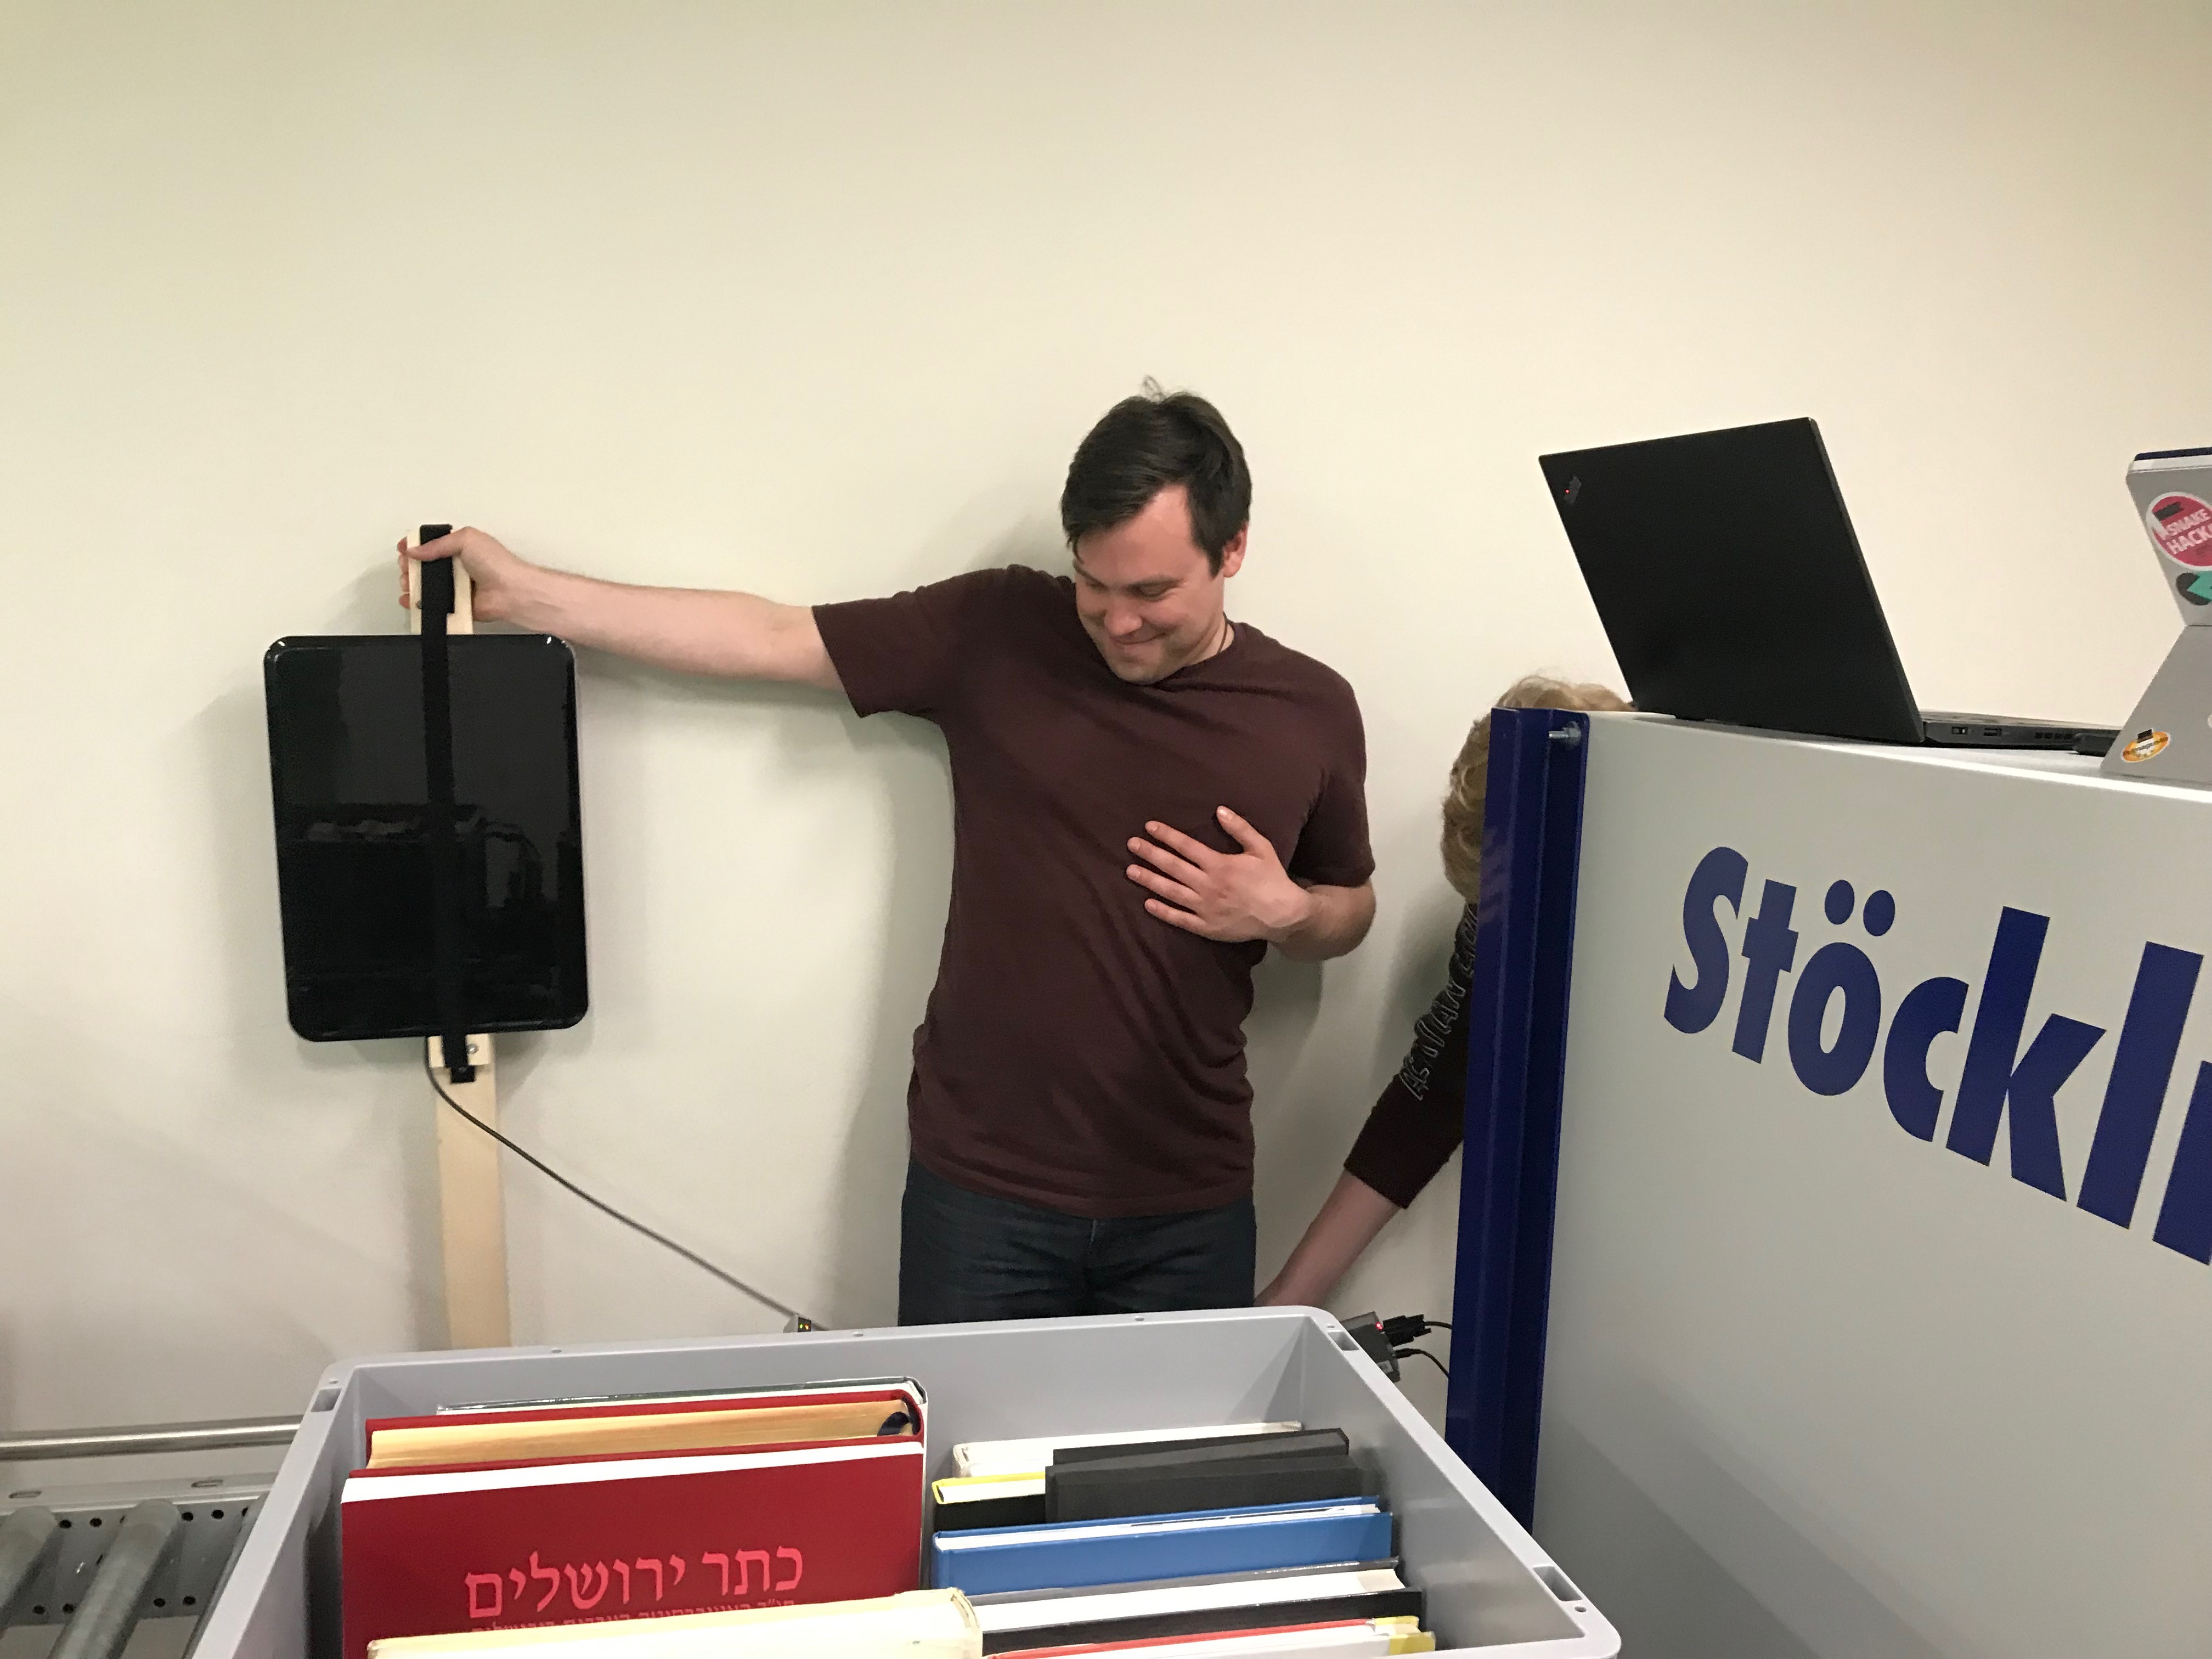
\includegraphics[keepaspectratio,width=\textwidth]{img/Testaufbau.jpg}
	\caption{Teammitglied Baumann beim Aufbau und Ausweichen von sensitiver Sensorik}
	\label{fig:AufbauSensorik}
\end{figure}

\section{Inbetriebnahme}
Sobald die Antennen plaziert waren, konnte mit der Inbetriebnahme fortgefahren werden. Schnell wurde klar, dass die Software geändert werden musste, da viele Tags nicht ausgelesen werden konnten und eine Exception warfen, welche nicht abgefangen wurde. Das Team entschied sich diese Exception zwar im Log festzuhalten, aber nicht weiter zu beachten. Danach konnte ein erstes Erfolgserlebnis erreicht werden, indem verifiziert werden konnte, dass die Ermittlung der Behälter über eine Mehrzahl der ExemplarIDs funktionierte.

\section{Test Multiple Tags}
Danach wurde getestet, wieviel Tags im Durchschnitt gelesen werden konnte. Die zwei häufigsten Layouts welche im Datensatz anzutreffen waren, waren das Layout L04 und L08 (siehe Abbildung \ref{fig:Layouts}), dennoch konnten anfangs nur durchschnittlich etwa 5 Tags pro Behälter gelesen werden. Das Team identifizierte dafür die Gründe, dass die Bücher zu dicht gestapelt waren und die RFID Tags immer etwa auf gleicher Höhe angebracht waren, plus die Reichweite der Antennen die nicht die ganzen Behälter abdecken konnten.

\begin{figure}[htb]
	\centering
	\begin{subfigure}{0.48\linewidth}
		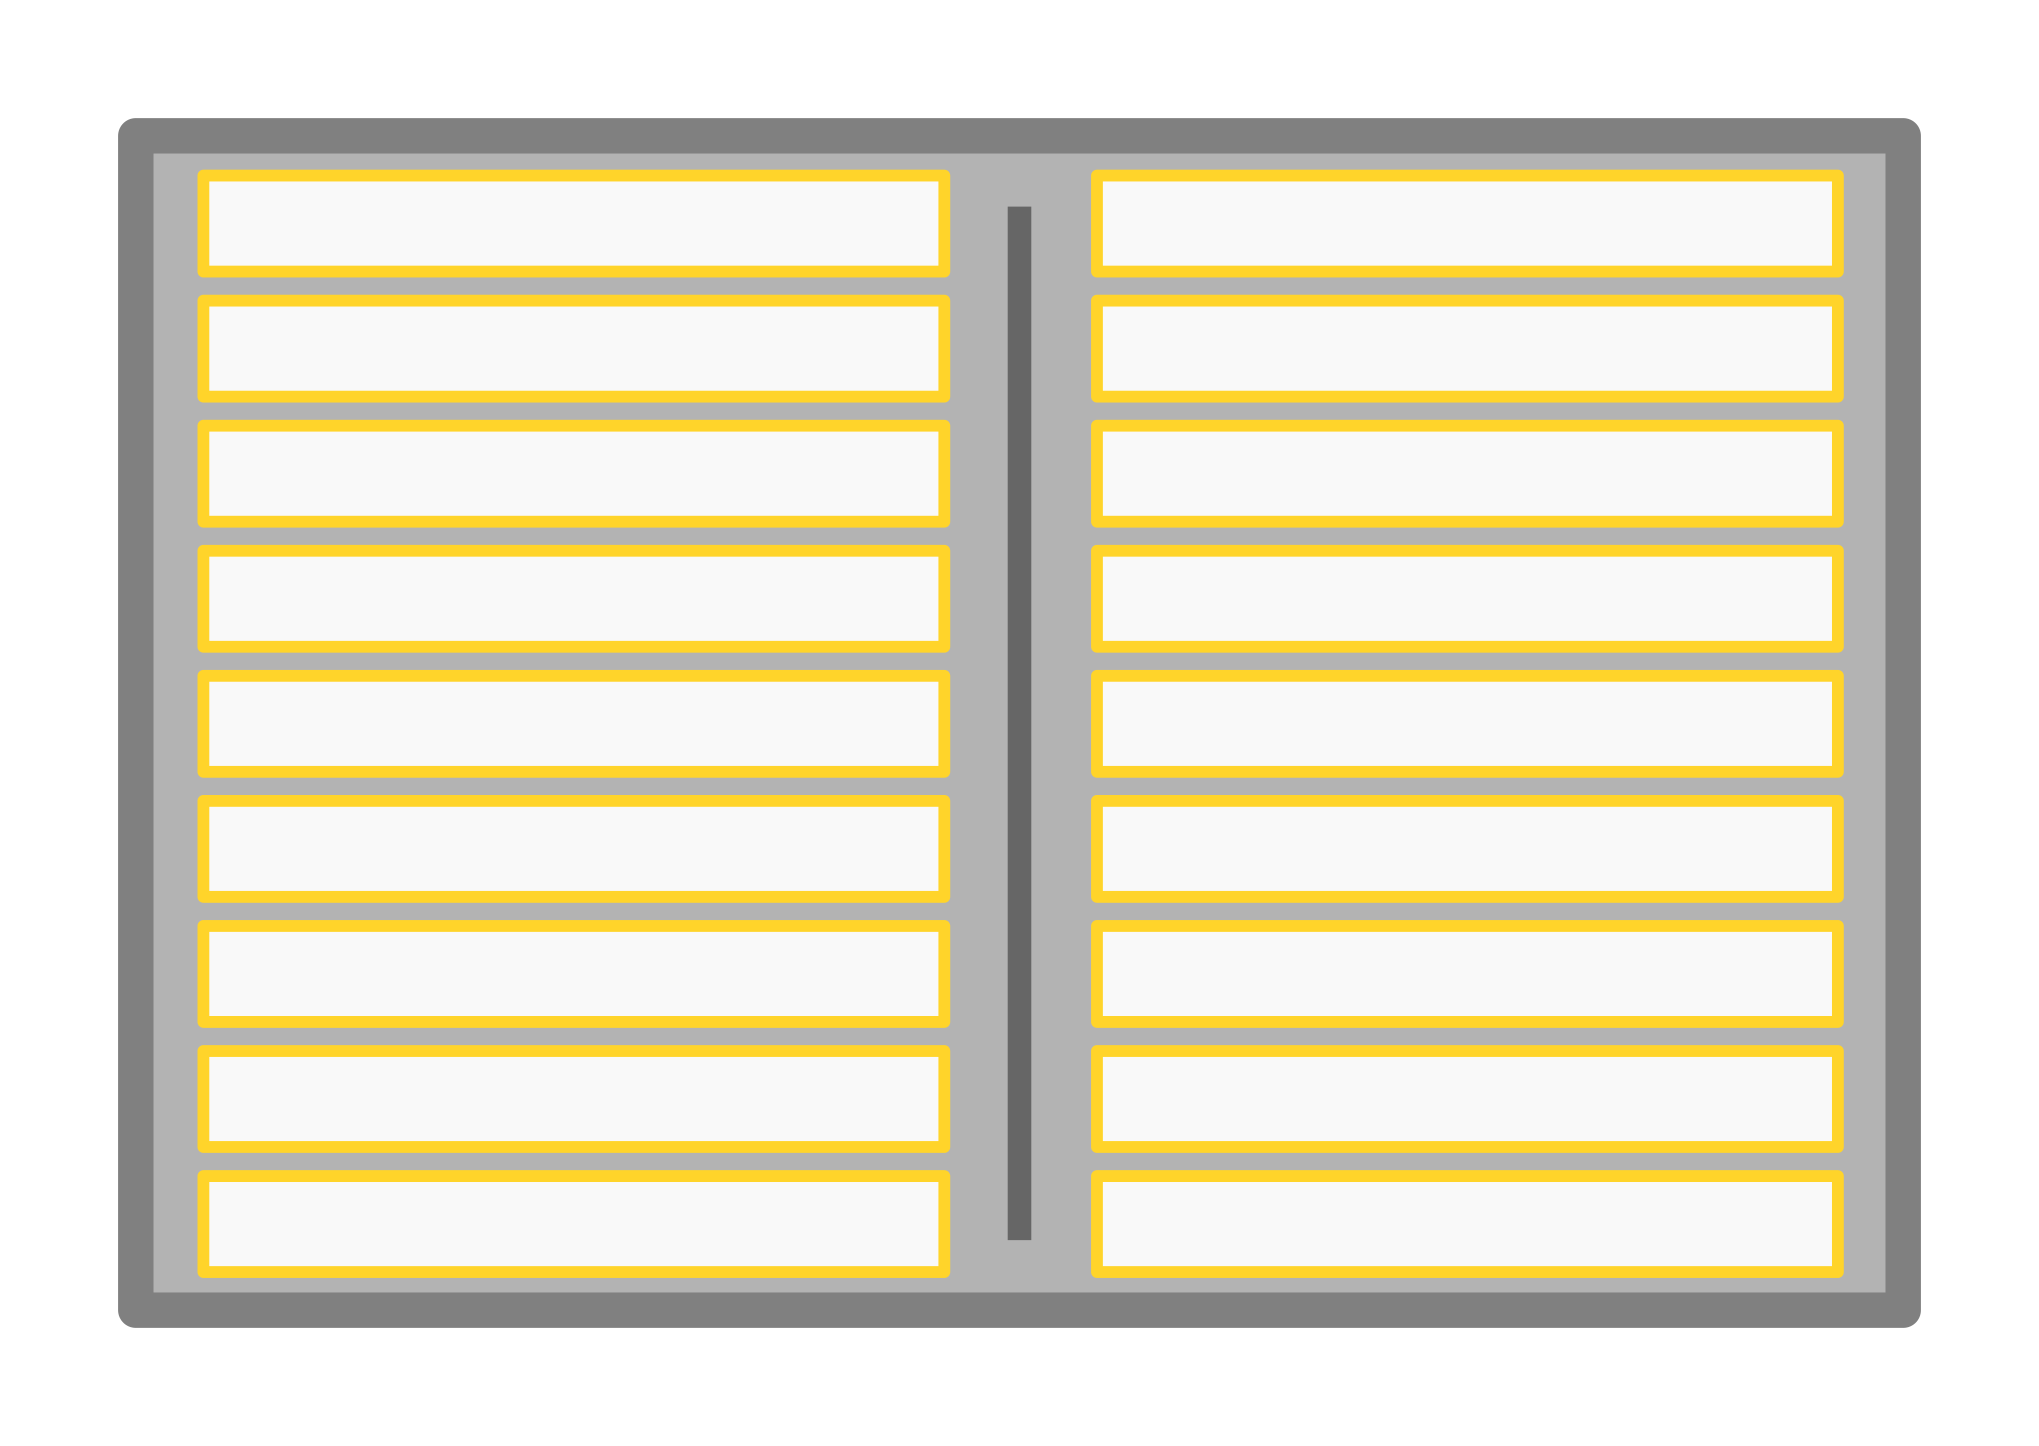
\includegraphics[keepaspectratio,width=\linewidth]{img/Layout04.png}
		\caption{Layout L04}
	\end{subfigure}
	\begin{subfigure}{0.48\linewidth}
		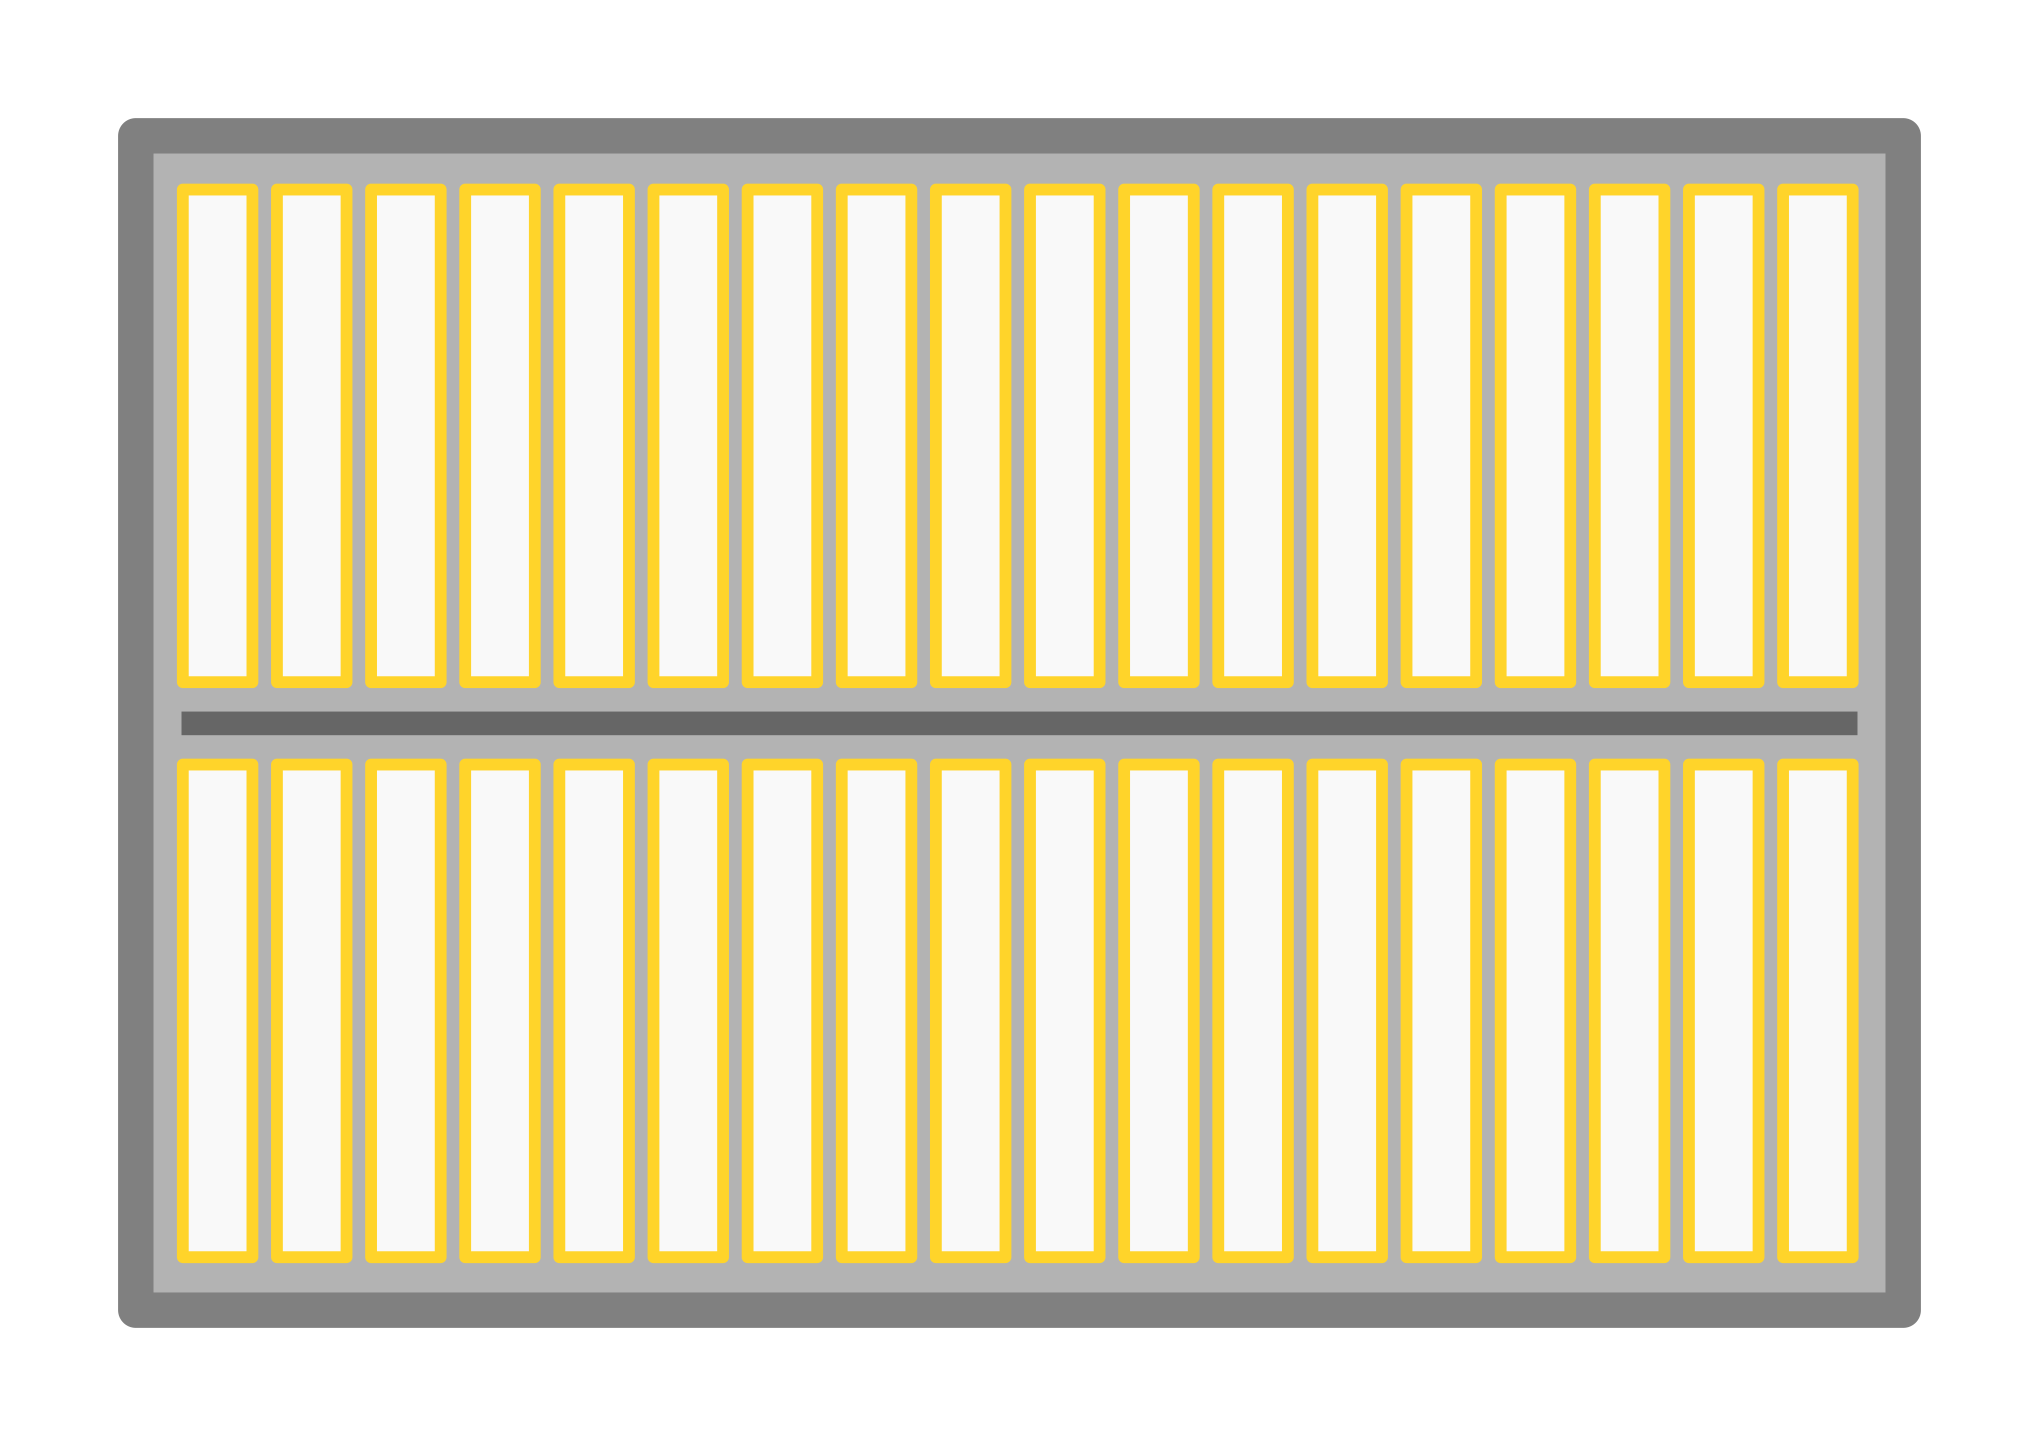
\includegraphics[keepaspectratio,width=\linewidth]{img/Layout08.png}
		\caption{Layout L08}
	\end{subfigure}
	\caption{Die zwei häufigsten Layouts}
	\label{fig:Layouts}
\end{figure}

\section{Test Vollbetrieb}
Der nächste Test welcher durchgeführt wurde war, wie gut die Applikation mit der vollen Geschwindigkeit des Förderbandes zurecht kommt. Es konnte in diesem Test einerseit ermittelt werden, dass bei der Eckpartie nie zwei Behälter nebeneinander zu liegen kommen, da der nächste Behälter in einer Warteposition vorher bleibt, bis der vordere Behälter auf der Waage zu liegen kommt (siehe Abbildung \ref{fig:PlanEckpartie}). Die beiden Behälter überschneiden sich jedoch wenn sie aneinander vorbeifahren (siehe Abbildung \ref{fig:AblaufEckpartie}). Weiter musste aufgrund der Geschwindigkeit des Auslesen der Behälter-Exemplar-Rückbeziehung die .csv-Datei in den Arbeitsspeicher geladen werden, da ansonsten die Berichterstattung viel zu langsam war.

\begin{figure}[htb]
	\centering
	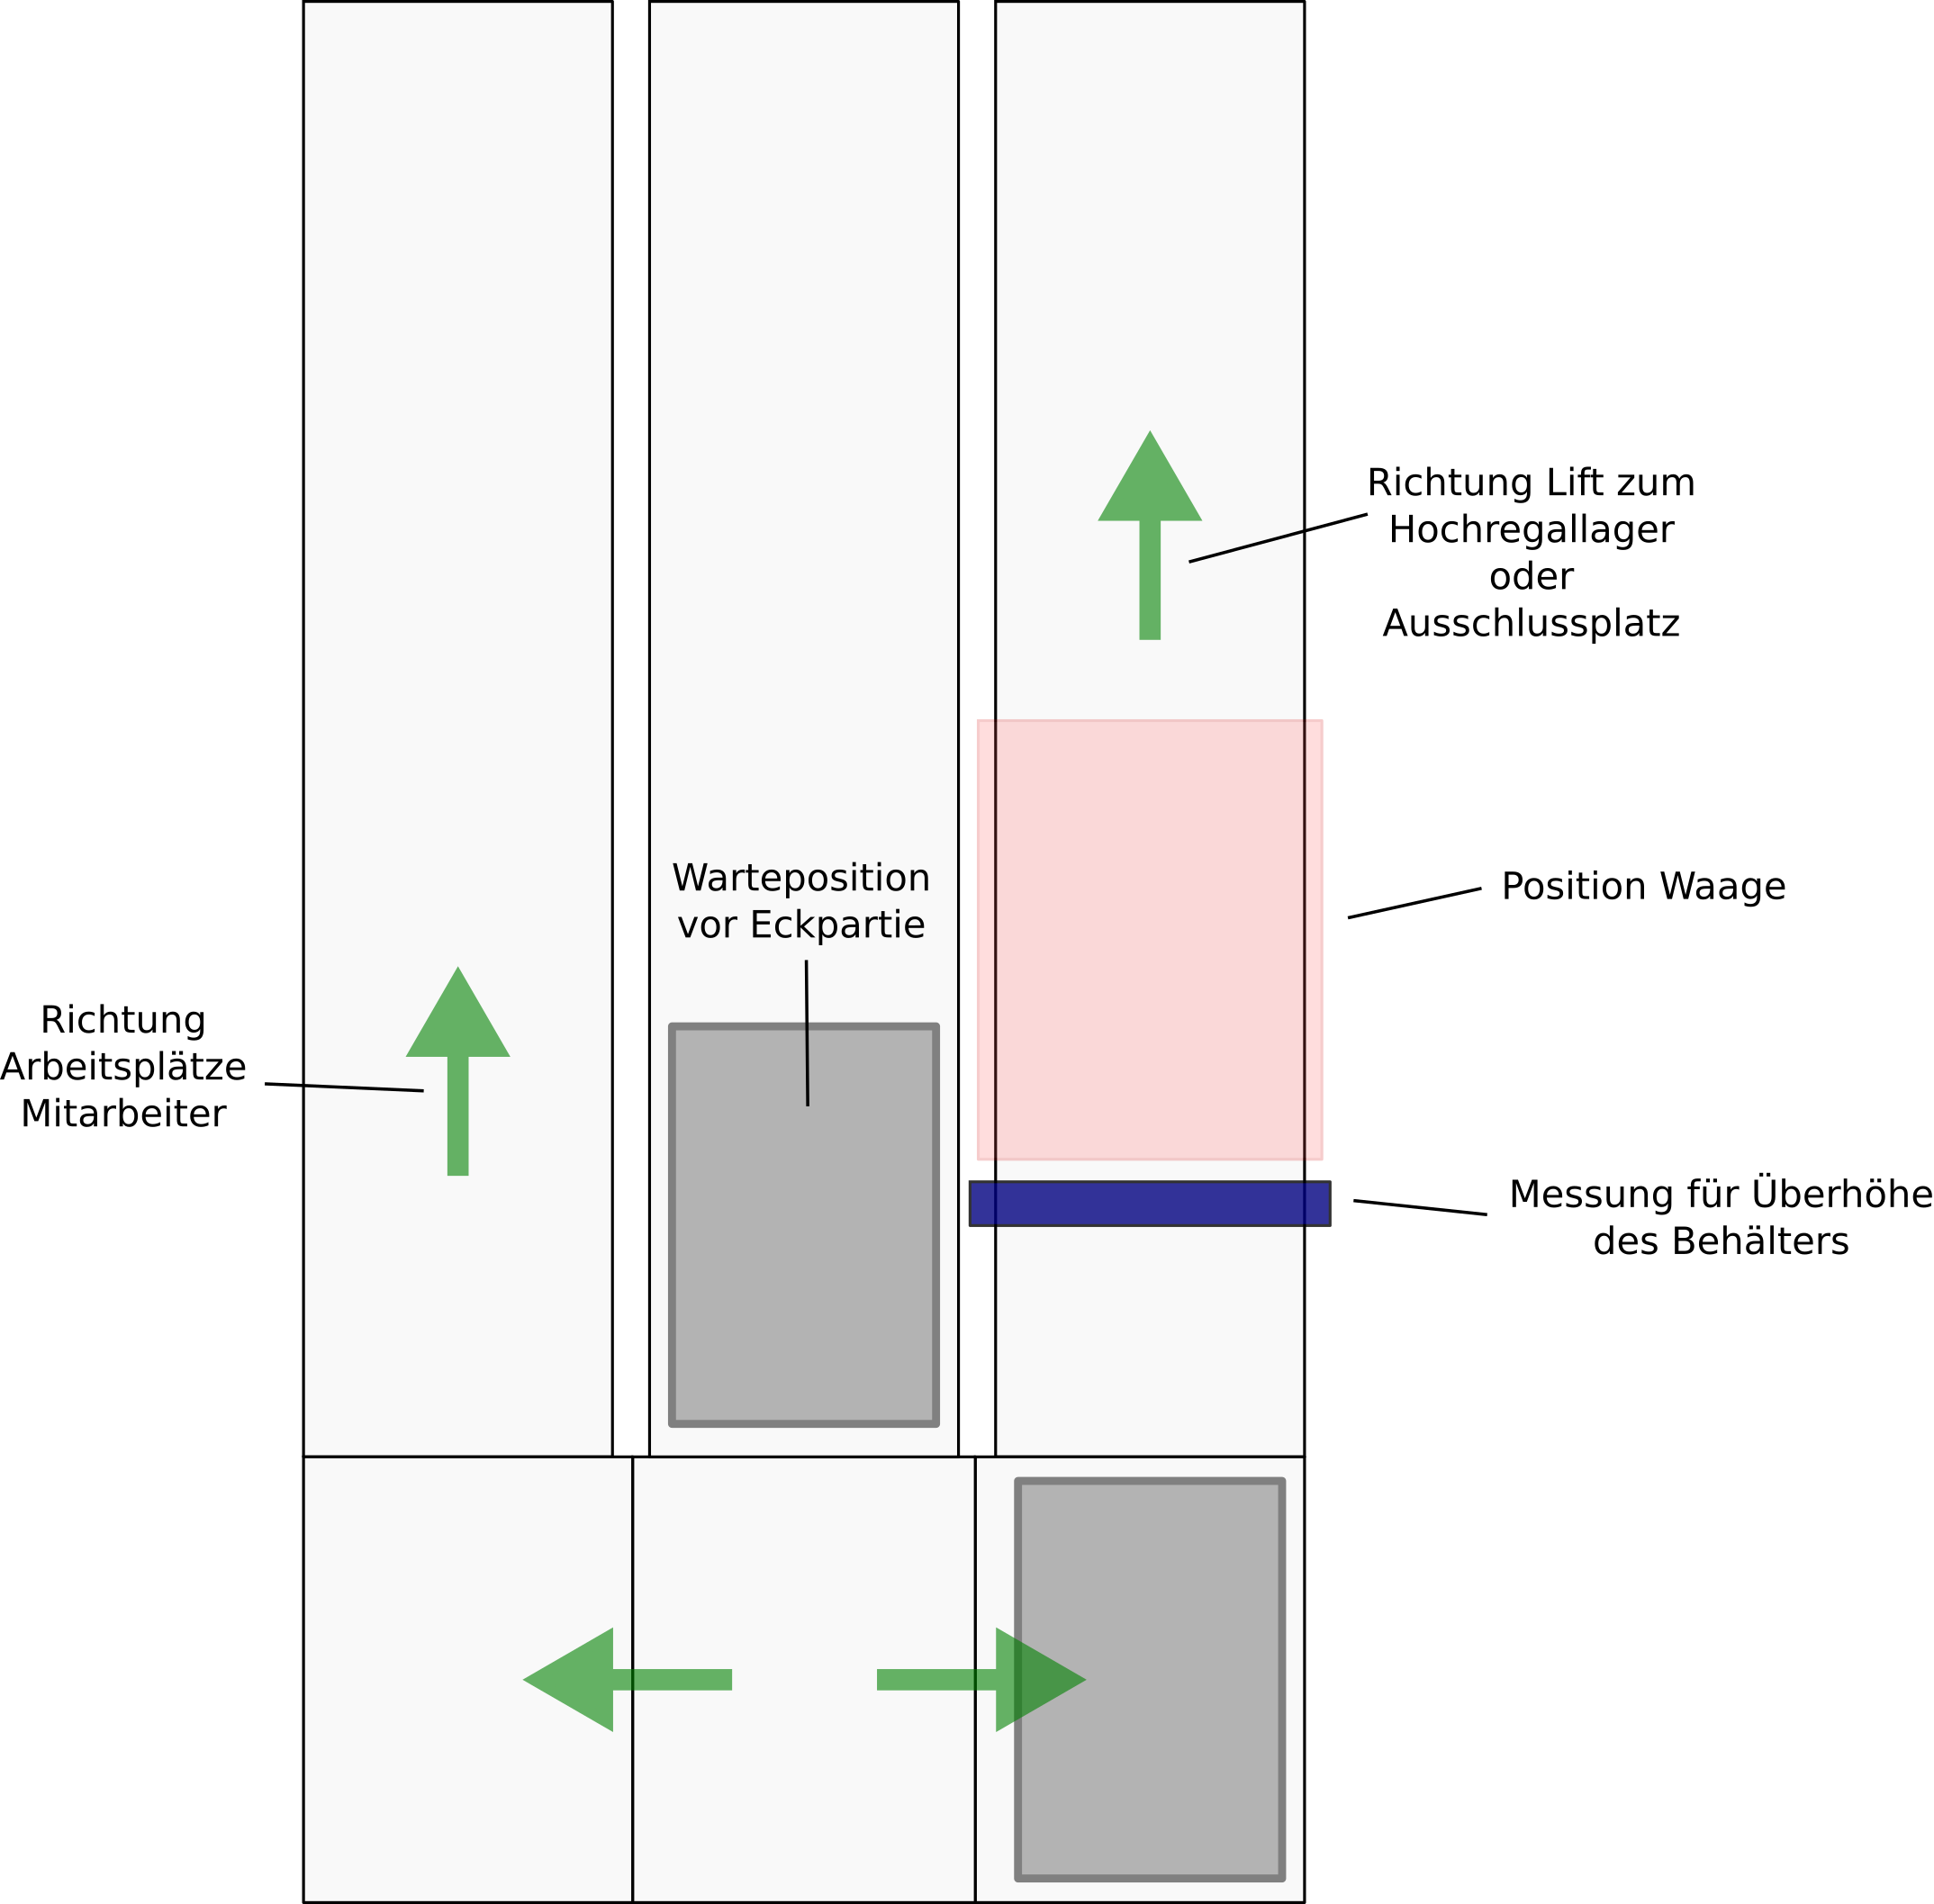
\includegraphics[keepaspectratio,width=0.6\linewidth]{img/PlanEckpartie.png}
	\caption{Lageplan mit Fokus auf die Eckpartie in der der Test durchgeführt wurde}
	\label{fig:PlanEckpartie}
\end{figure}

\begin{figure}[htb]
	\centering
	\begin{subfigure}{0.3\linewidth}
		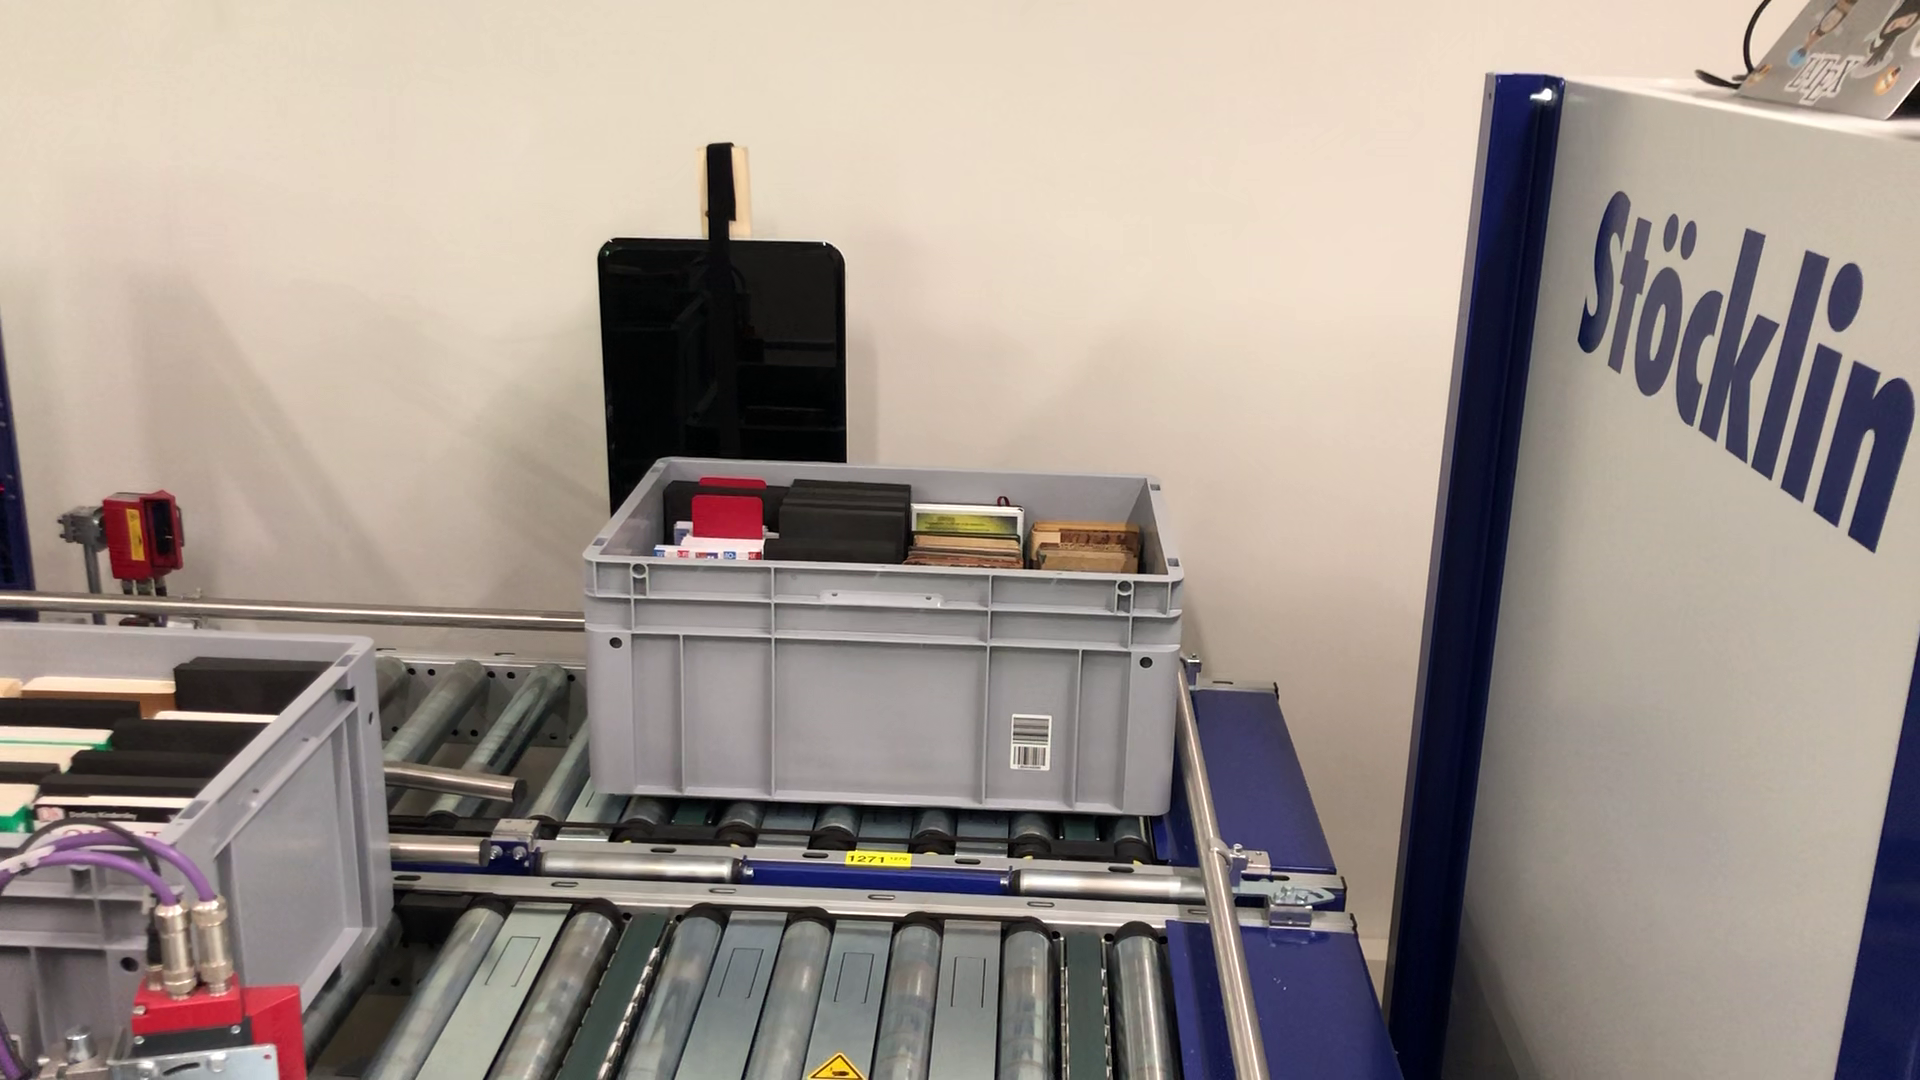
\includegraphics[keepaspectratio,width=\linewidth]{AblaufEckpartie01.png}
	\end{subfigure}
	\begin{subfigure}{0.3\linewidth}
		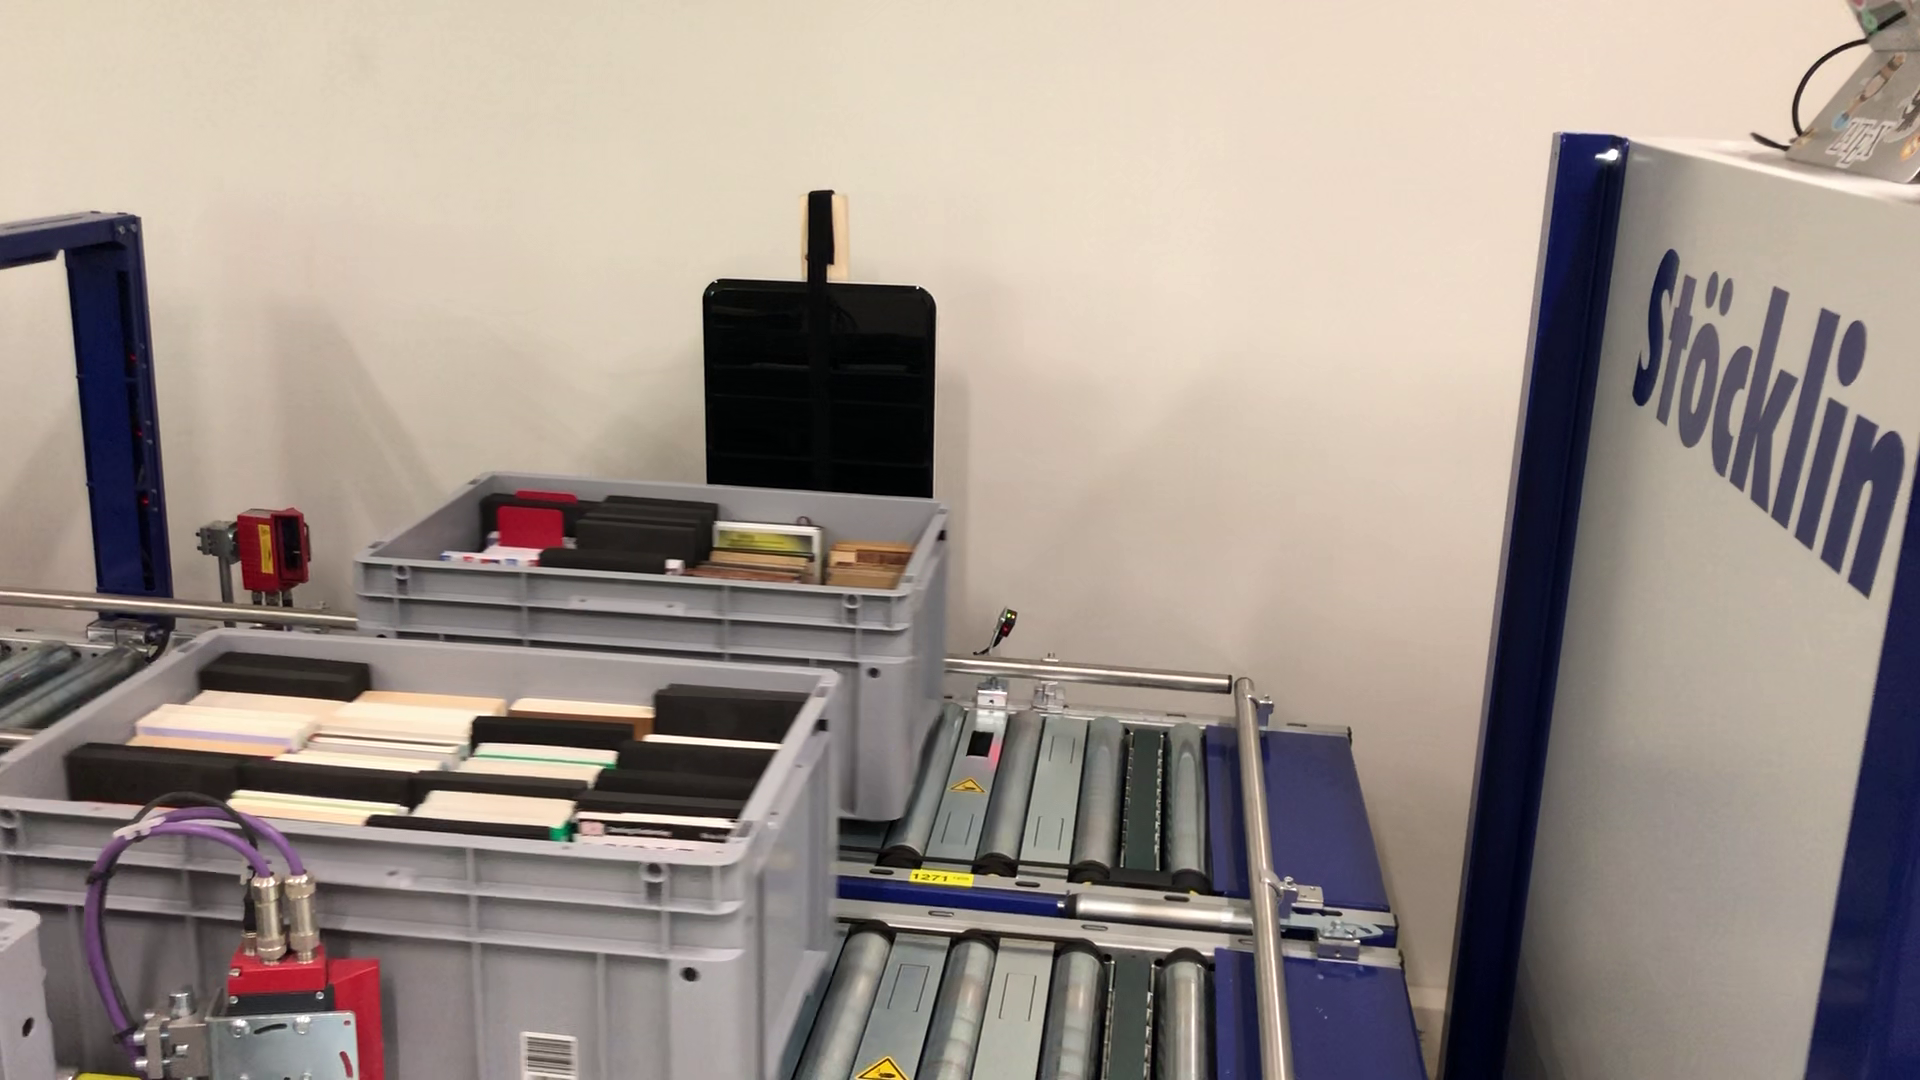
\includegraphics[keepaspectratio,width=\linewidth]{AblaufEckpartie02.png}
	\end{subfigure}
	\begin{subfigure}{0.3\linewidth}
		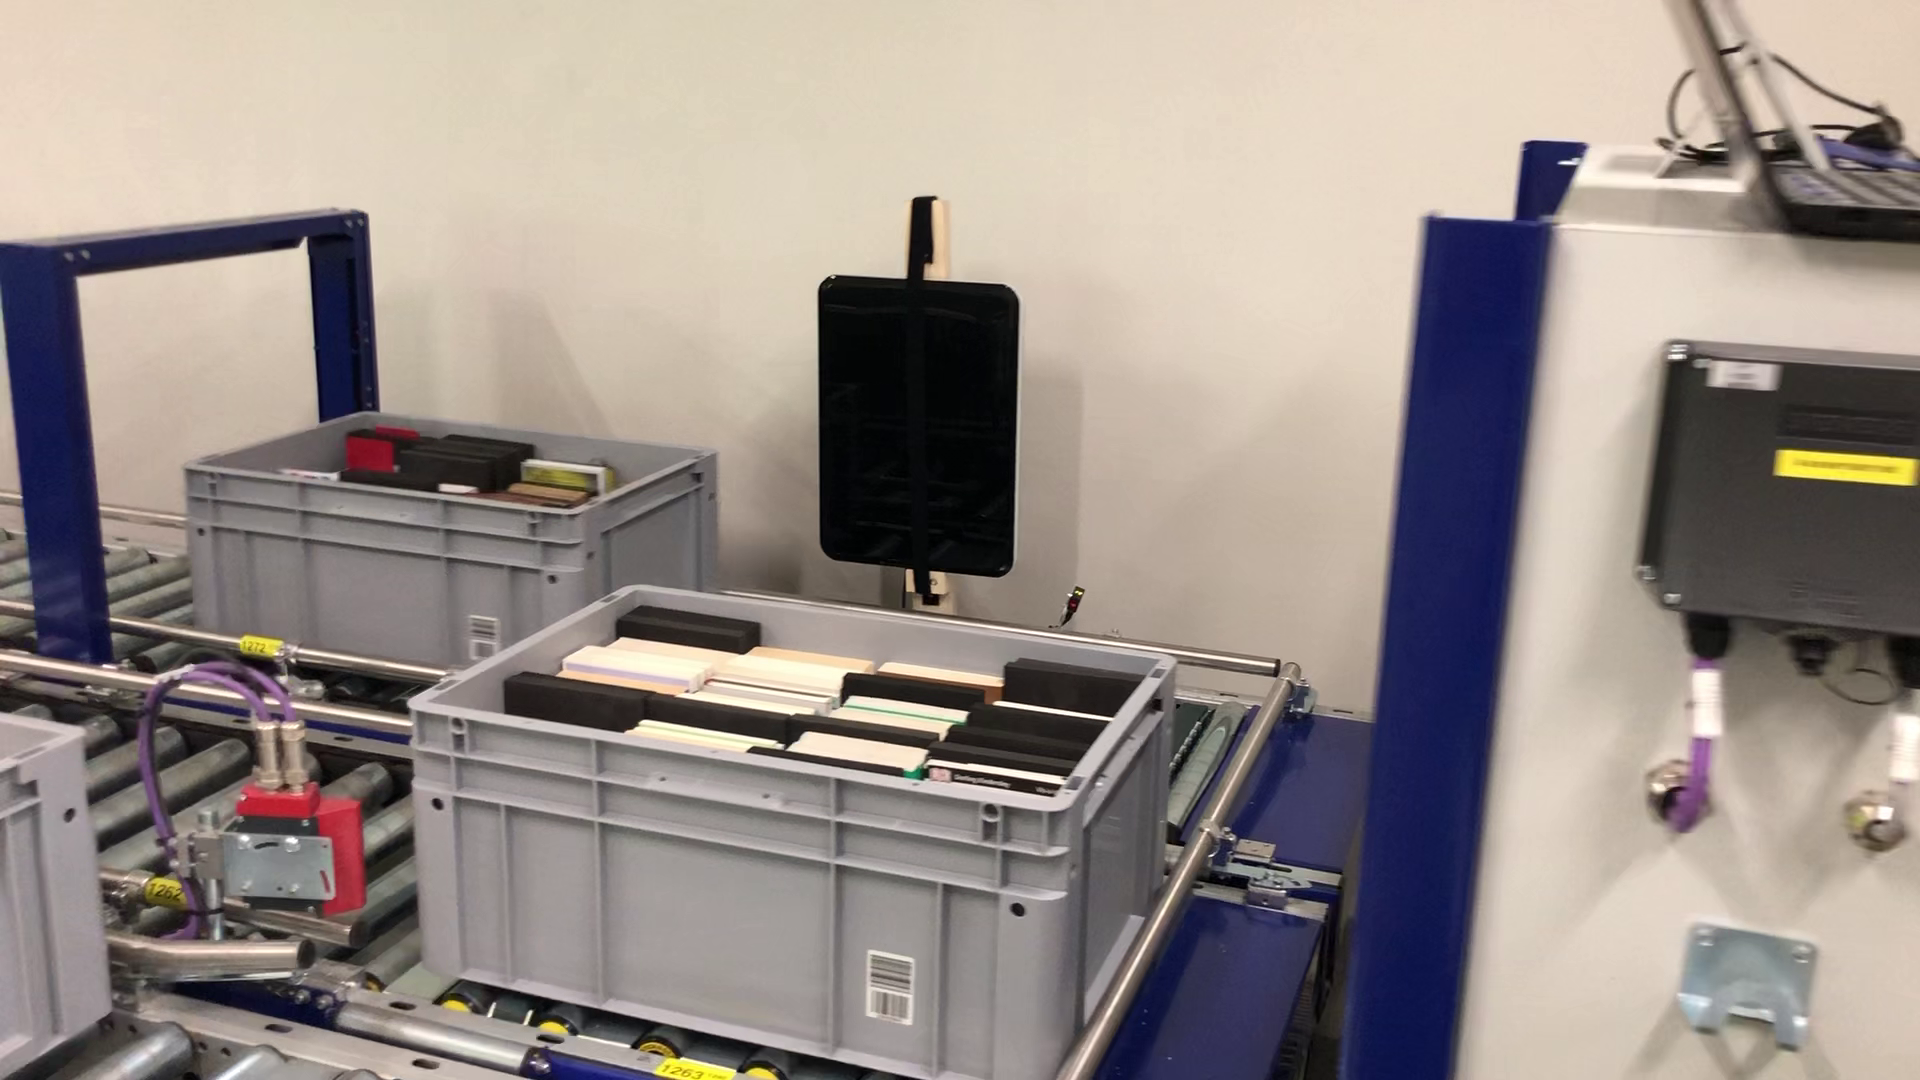
\includegraphics[keepaspectratio,width=\linewidth]{AblaufEckpartie03.png}
	\end{subfigure}
	\caption{Ablauf der Bewegung in der Eckpartie bei Vollbetrieb}
	\label{fig:AblaufEckpartie}
\end{figure}

\section{Test Antennenposition}
Weiter wurde mit verschiedenen Antennenpositionen experimentiert, unter anderem bei der Position der Waage und in der Eckpartie (siehe Abbildung \ref{fig:PlanEckpartie}). Es konnte ermittelt werden, dass das Auslesen bei der Eckpartie besser funktioniert als die bei der Waage der Fall ist, da sich der Behälter länger im Lesebereich der Antenne befindet. Weiter konnte eruiert werden, dass die Antenne in horizontaler Ausrichtung mehr Tags auslesen kann, als in vertikaler Ausrichtung (siehe Abbildung \ref{fig:AusrichtungAntenne}).

\begin{figure}[htb]
	\centering
	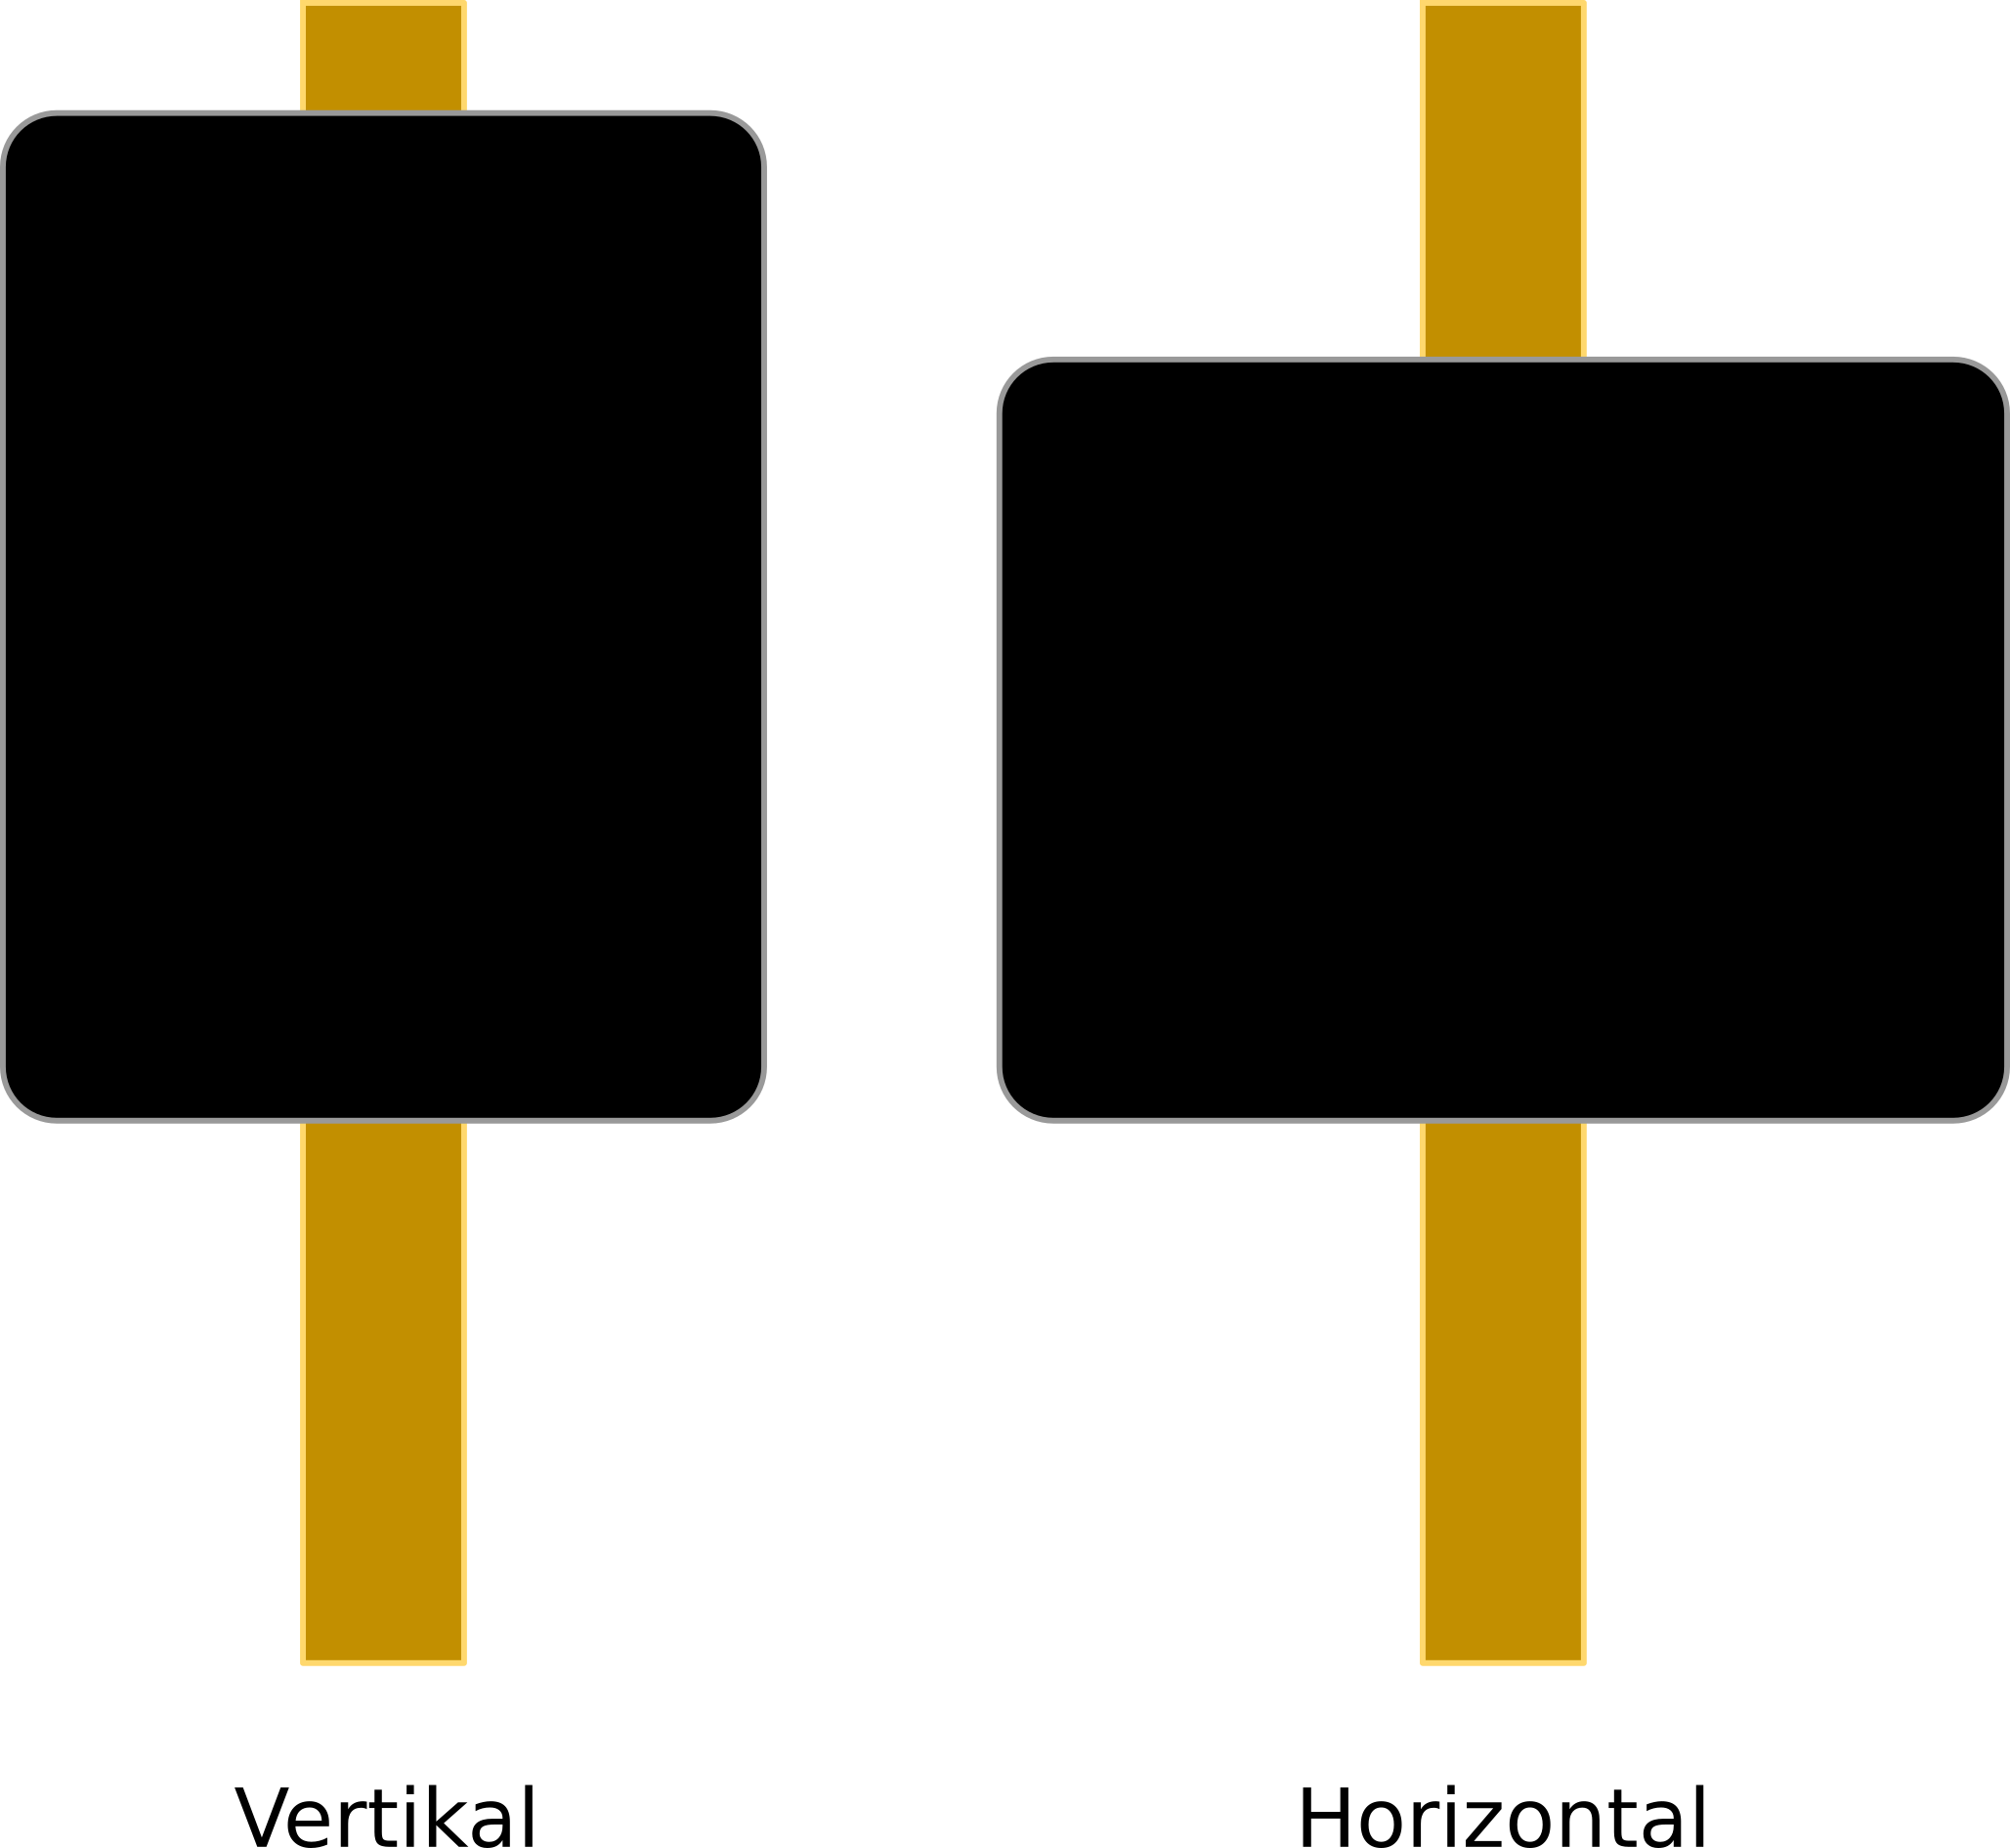
\includegraphics[keepaspectratio,width=0.6\linewidth]{img/AusrichtungAntenne.png}
	\caption{Ausrichtungsarten der Antenne in Referenz zur Halterung}
	\label{fig:AusrichtungAntenne}
\end{figure}

\begin{figure}[htb]
	\centering
	\includegraphics[keepaspectratio,width=0.6\linewidth]{img/FinaleAntennenPosition.png}
	\caption{Position der Antennen bis zum Schluss der Tests}
	\label{fig:FinalePositionAntennen}
\end{figure}

\section{Test Deplatziertes Exemplar}
Anschliessend wurde mit einem eigens mitgebrachten Tag, dass erkennen eines deplazierten Exemplars getestet. Dies wurde von der Applikation erkannt, sofern dieser Tag die Bedingungen erfüllt um Ihn auslesen zu können. Dies beinhaltet, dass eine gewise Distanz zu Anderen Tags eingehalten wird, sowie die Ausrichtung des Tags zur Antenne den kritischen Wert nicht übersteigt. Auf der Abbildung \ref{fig:PositionenRFIDTag} wird dargestellt, bei welchen Szenarien der Test erfolgreich war und bei welchen nicht.

\begin{figure}[htb]
	\centering
	\begin{subfigure}{0.48\linewidth}
		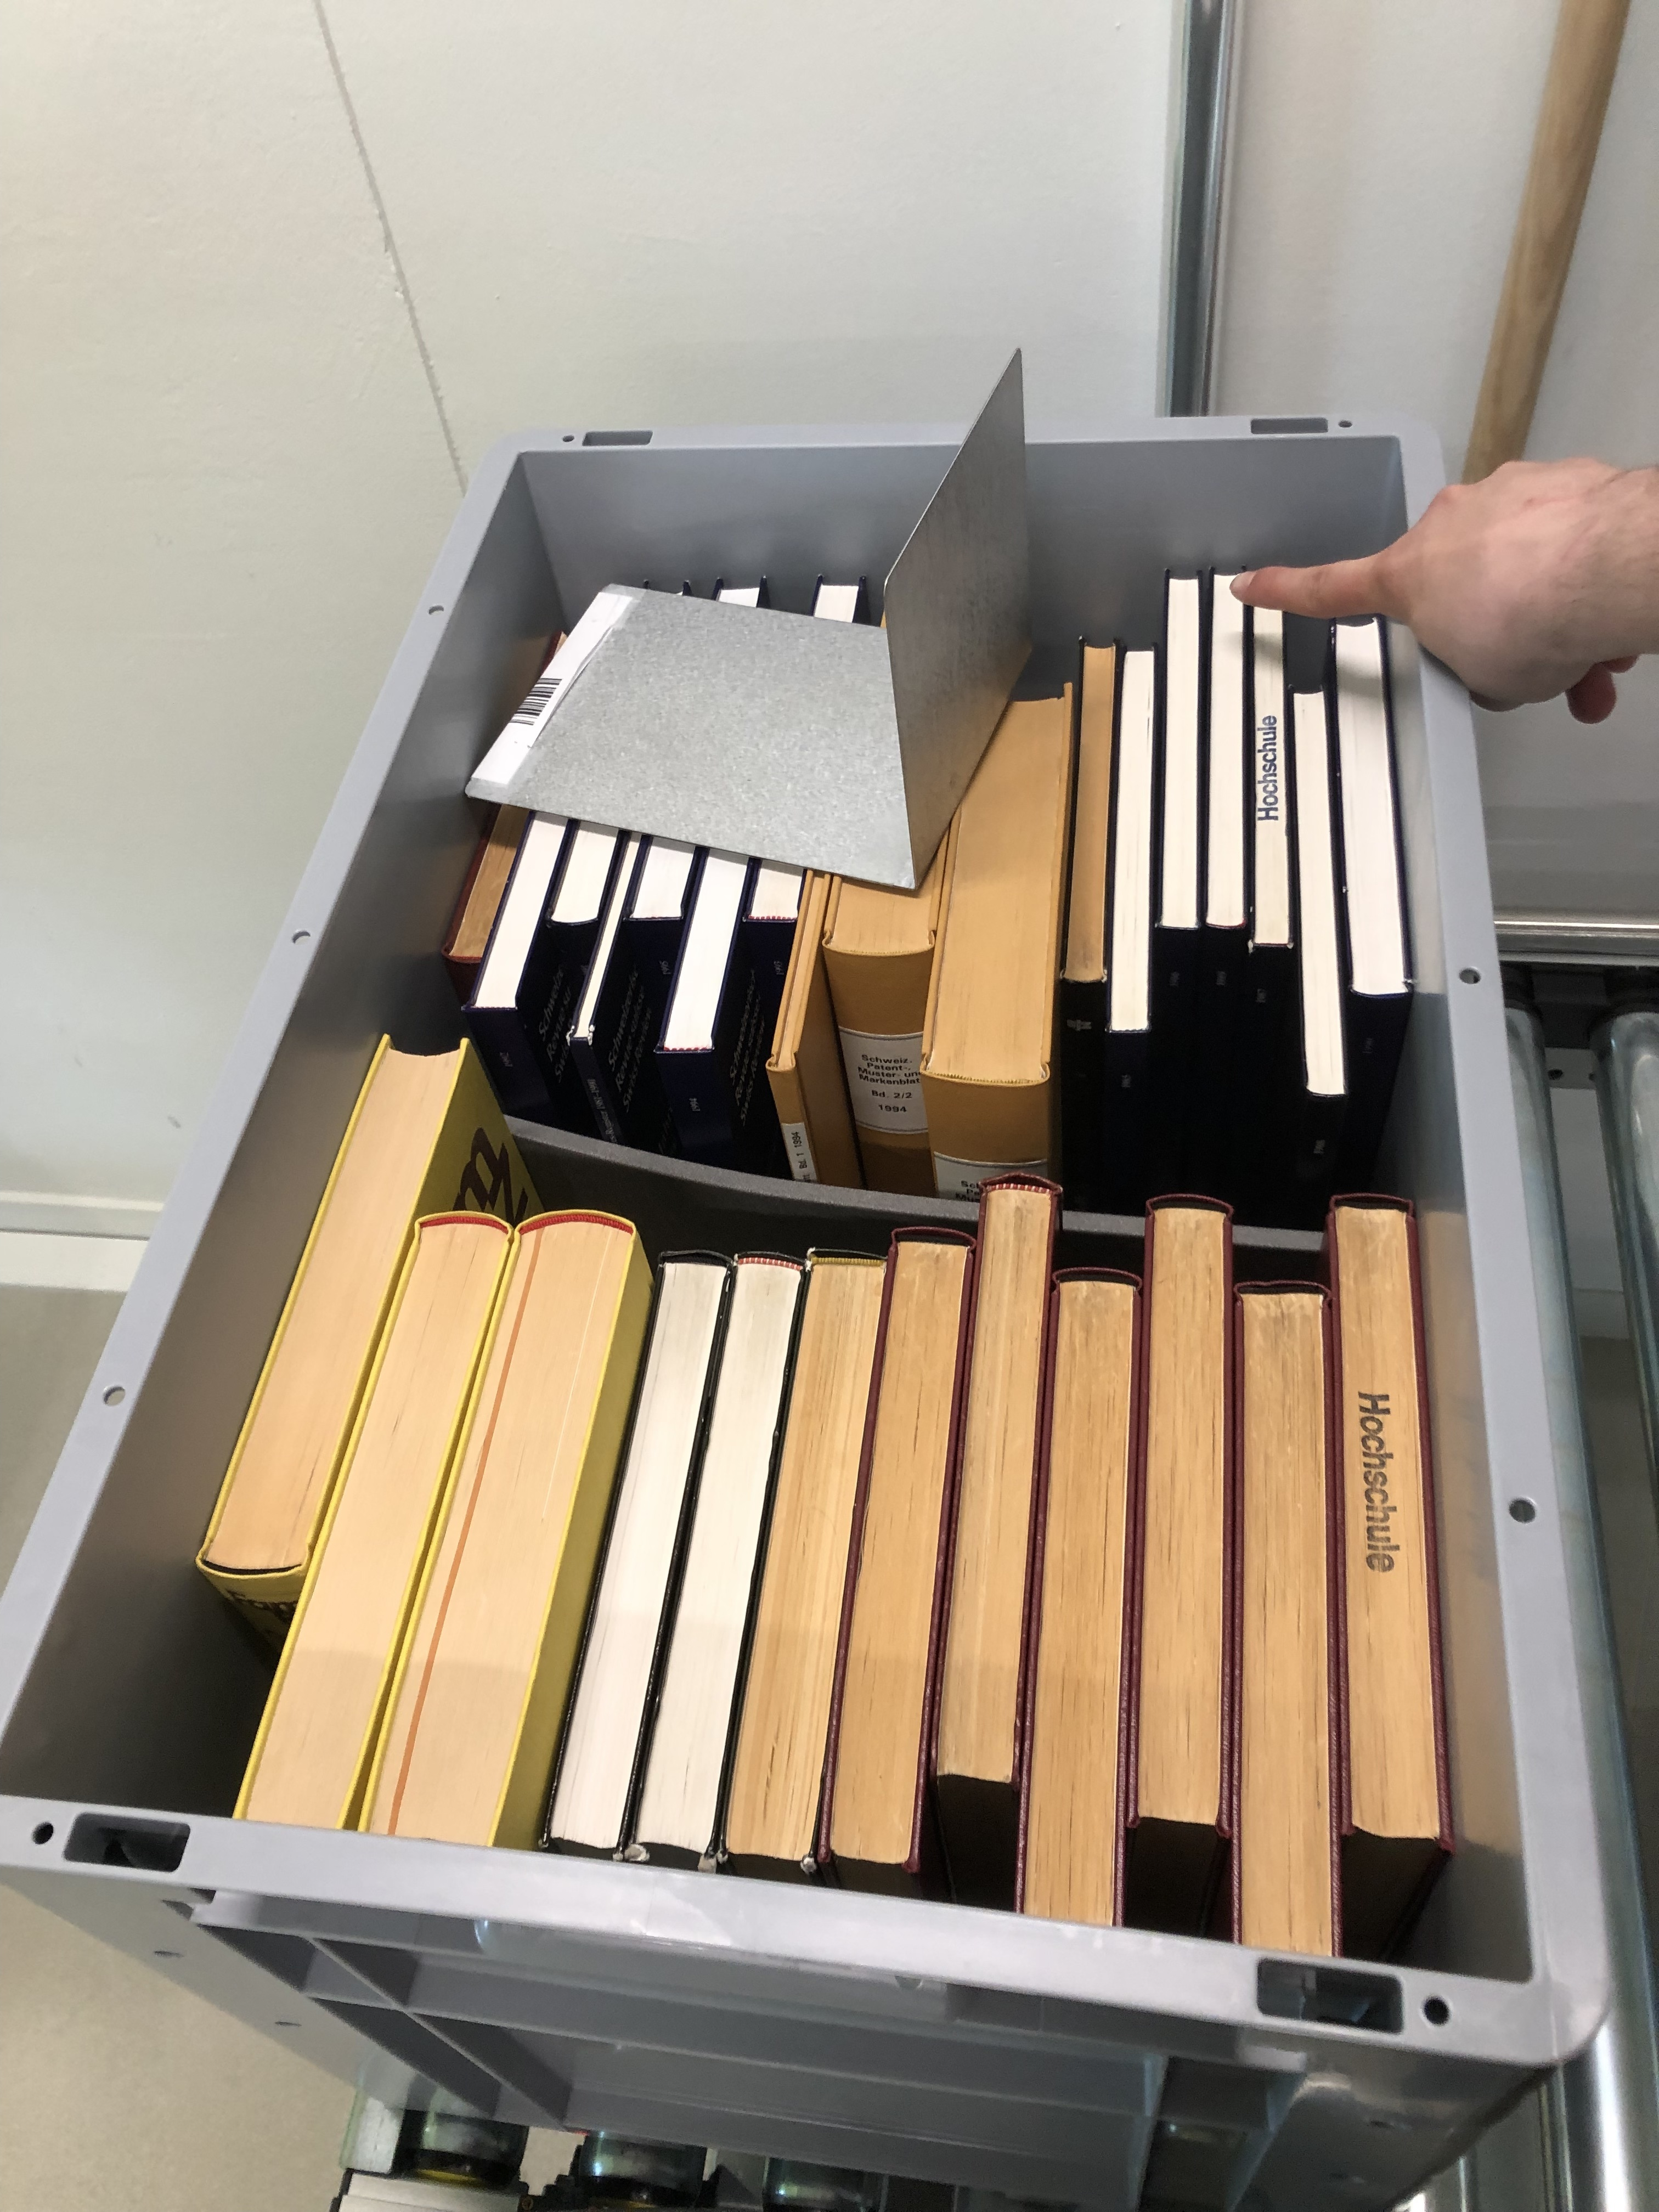
\includegraphics[keepaspectratio,width=\linewidth]{img/RFIDPositionErfolgreich.jpg}
		\caption{Position des RFID Tags bei erfolgreichen Erkennungen}
	\end{subfigure}
	\begin{subfigure}{0.48\linewidth}
		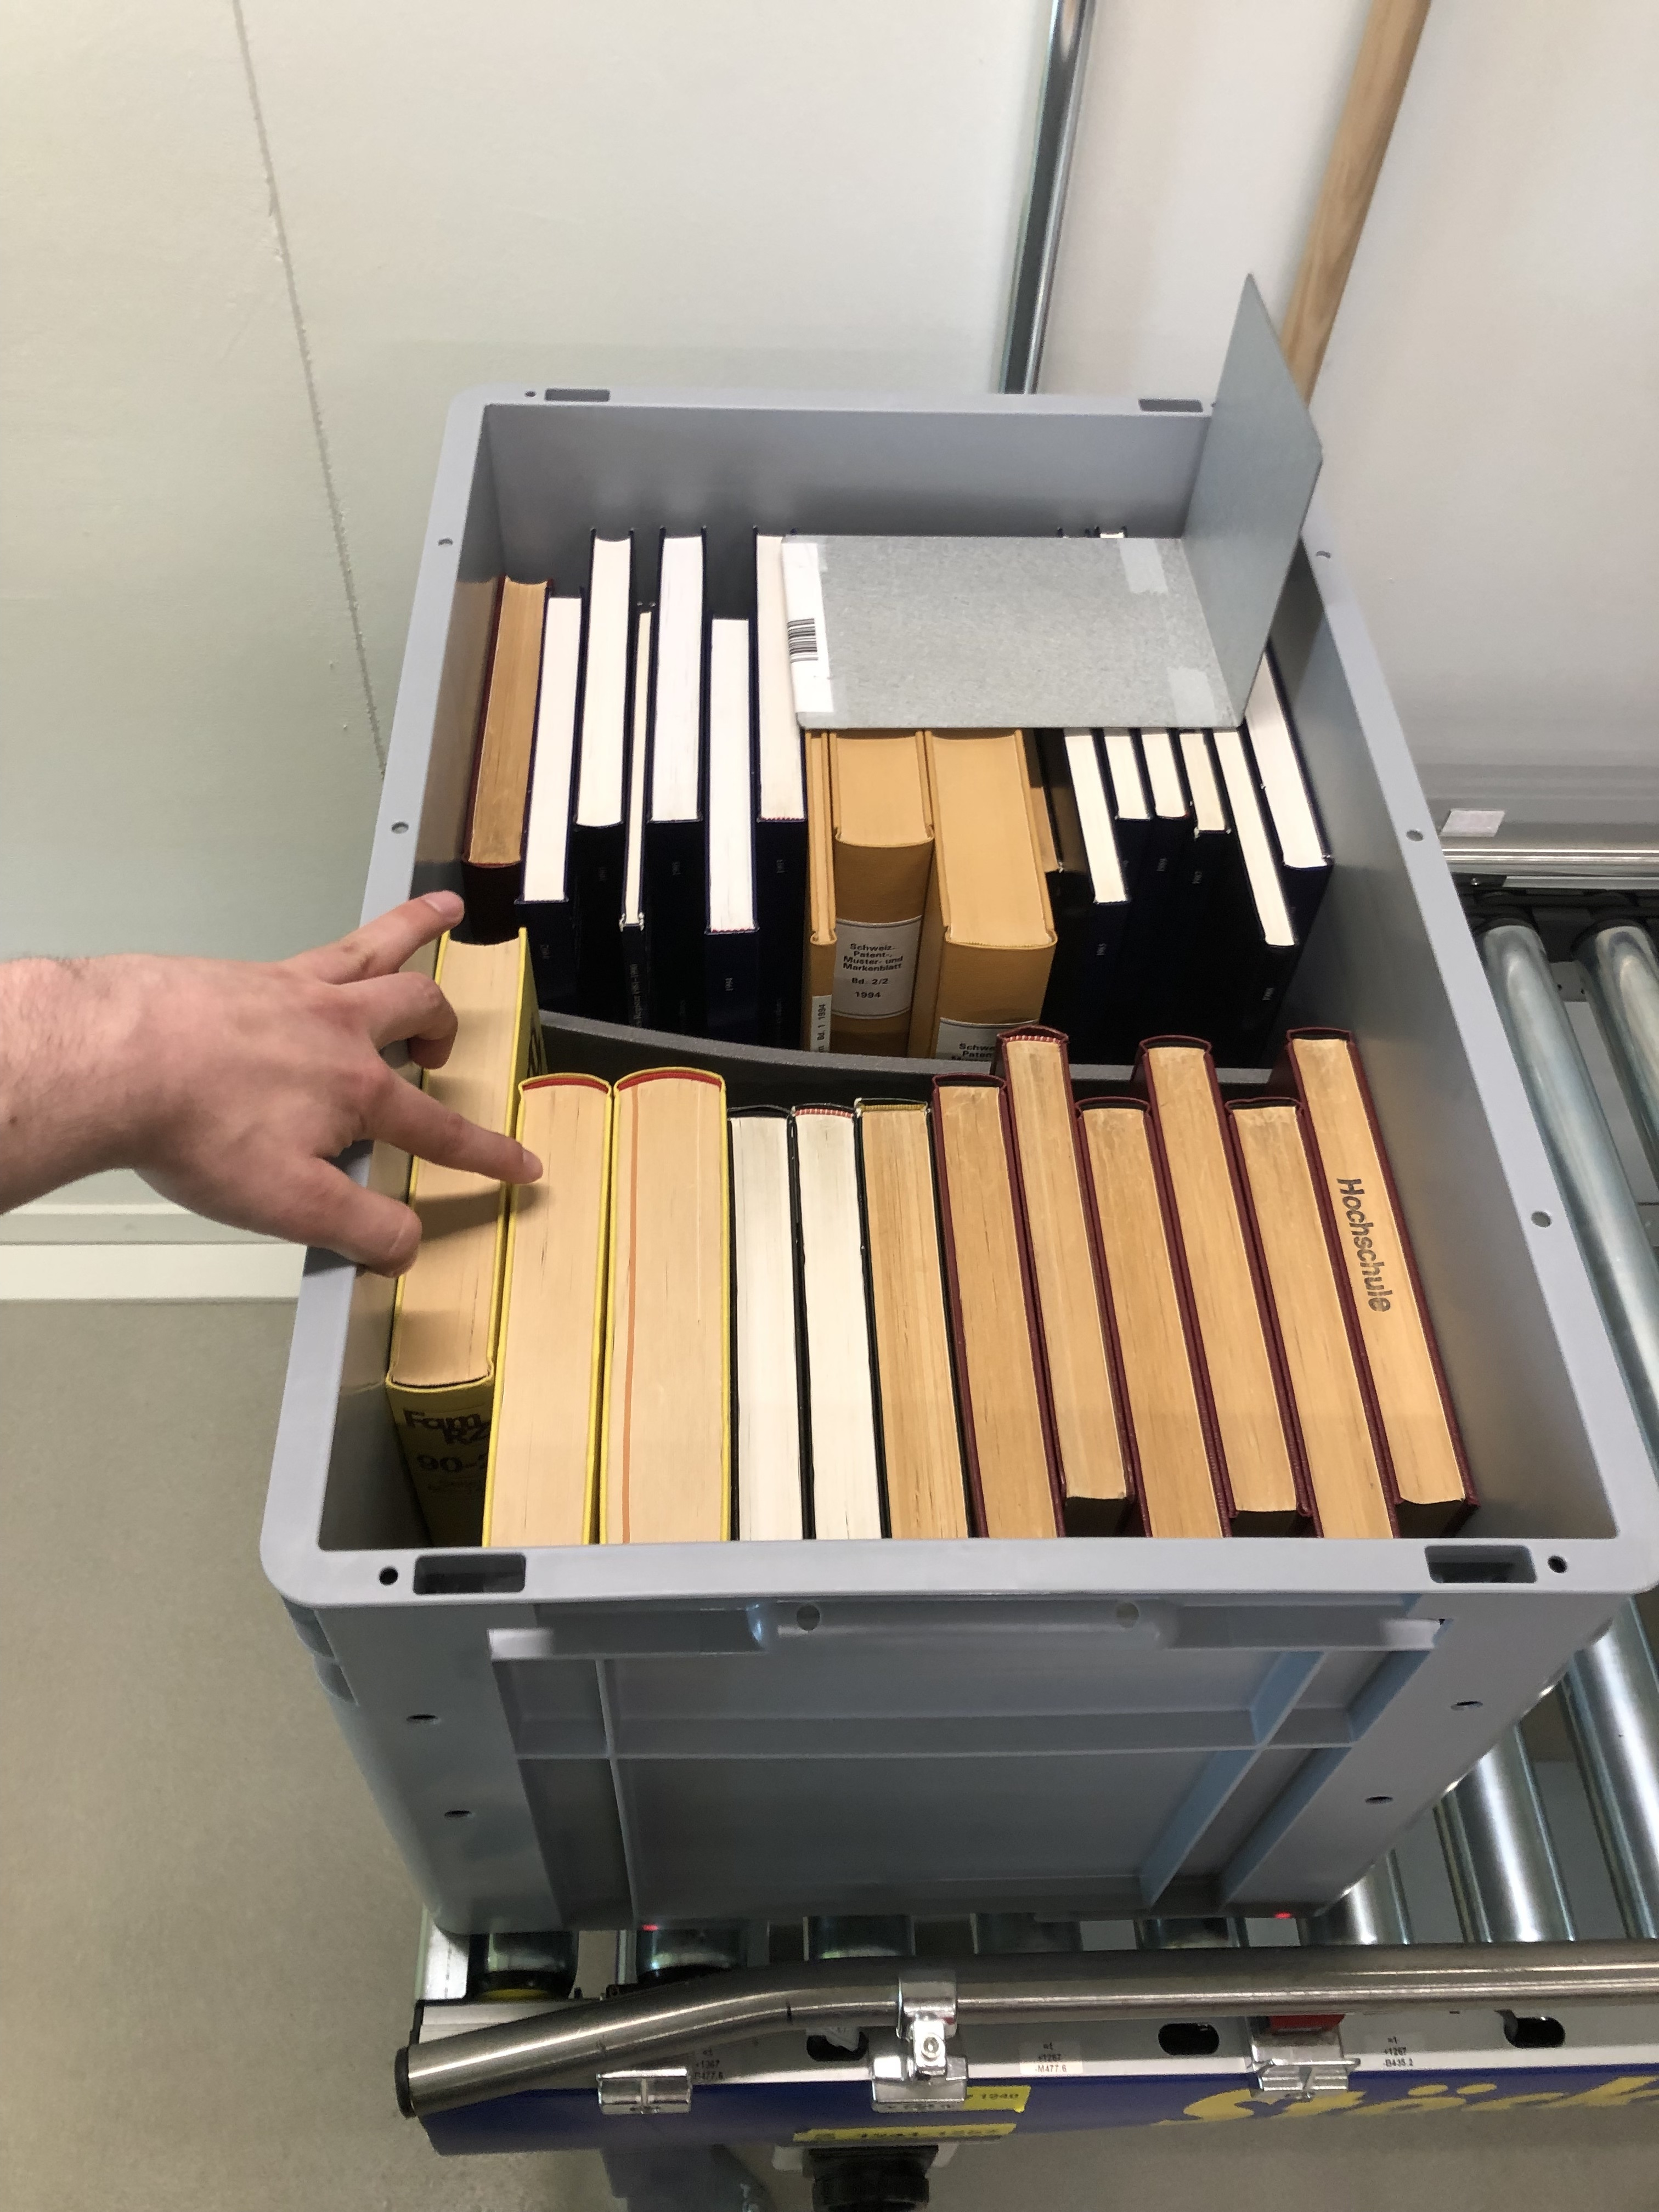
\includegraphics[keepaspectratio,width=\linewidth]{img/RFIDPositionNichtErfolgreich.jpg}
		\caption{Position des RFID Tags bei nicht erfolgreichen Erkennungen}
	\end{subfigure}
	\caption{Positionen RFID Tag}
	\label{fig:PositionenRFIDTag}
\end{figure}

\section{Auslesegeschwindigkeit}
Der Behälter befand sich etwa drei Sekunden im Lesebereich beider Antennen. Im Test wurden im Maximum 27 ExemplarIDs erfolgreich ausgelesen. Dies ergibt eine maximal erreichte Leserate von $9 \frac{ExemplarIDs}{Sekunde}$.

\clearpage

\begin{lstlisting}
<record>
<date>2019-05-28T06:35:20</date>
<millis>1559050520265</millis>
<sequence>1638</sequence>
<logger>RFIDReferenzimplementation</logger>
<level>INFO</level>
<class>
	ch.bda.baumannwicki.misplacedtagidentifier.log.LogPersistorImpl
</class>
<method>printTagsFound</method>
<thread>9</thread>
<message>
	LibraryCopies found: [
		ArticleID: ILUM02142955, BoxID: LB00040204,
		ArticleID: ILUM02142950, BoxID: LB00040204,
		ArticleID: ILUM02142951, BoxID: LB00040204,
		ArticleID: ILUM02142992, BoxID: LB00040204,
		ArticleID: ILUM02142971, BoxID: LB00040204,
		ArticleID: ILUM02146779, BoxID: LB00040204,
		ArticleID: ILUM02142956, BoxID: LB00040204,
		ArticleID: ILUM02142957, BoxID: LB00040204,
		ArticleID: ILUM02146786, BoxID: LB00040204,
		ArticleID: ILUM02146080, BoxID: LB00040204,
		ArticleID: ILUM02146081, BoxID: LB00040204,
		ArticleID: ILUM02146082, BoxID: LB00040204,
		ArticleID: ILUM02146927, BoxID: LB00040204,
		ArticleID: ILUM02146765, BoxID: LB00040204,
		ArticleID: ILUM02146941, BoxID: LB00040204,
		ArticleID: ILUM02146942, BoxID: LB00040204,
		ArticleID: ILUM02142949, BoxID: LB00040204,
		ArticleID: ILUM02146943, BoxID: LB00040204,
		ArticleID: ILUM02146767, BoxID: LB00040204,
		ArticleID: ILUM02142947, BoxID: LB00040204,
		ArticleID: ILUM02146704, BoxID: LB00040204,
		ArticleID: ILUM02146309, BoxID: LB00040204,
		ArticleID: ILUM02146770, BoxID: LB00040204,
		ArticleID: ILUM02146771, BoxID: LB00040204,
		ArticleID: ILUM02146772, BoxID: LB00040204,
		ArticleID: ILUM02142990, BoxID: LB00040204,
		ArticleID: ILUM02261706, BoxID: LB00040204
	]
</message>
</record>
\end{lstlisting}

\section{Fazit}
Die in den Versuchen emittelten Anforderungen zum erfolgreichen Lesen eines Tags, im Bezug auf die Reichweite, Ausrichtung zwischen Tag und Antenne und Distanz zwischen den Tags, konnten mit diesem Test bestätigt werden. Somit ist eine Identifikation der Behälter, wie auch der deplazierten Exemplaren, unter Einhaltung dieser Anforderungen, möglich. Dennoch sind Optimierungen in der Applikation möglich, sowie die Anschaffung der Geräte von Feig, zur Erreichung einer vollen Abdeckung der Behälter, nötig.

\end{document}
